% ******************************************************** %
%              TEMPLATE DE INFORME ORGA2 v0.1              %
% ******************************************************** %
% ******************************************************** %
%                                                          %
% ALGUNOS PAQUETES REQUERIDOS (EN UBUNTU):                 %
% ========================================
%                                                          %
% texlive-latex-base                                       %
% texlive-latex-recommended                                %
% texlive-fonts-recommended                                %
% texlive-latex-extra?                                     %
% texlive-lang-spanish (en ubuntu 13.10)                   %
% ******************************************************** %


\documentclass[a4paper]{article}
\usepackage[spanish]{babel}
\usepackage[utf8]{inputenc}
\usepackage{charter}   % tipografia
\usepackage{graphicx}
%\usepackage{makeidx}
\usepackage{paralist} %itemize inline
\usepackage{float}

%\usepackage{float}
%\usepackage{amsmath, amsthm, amssymb}
%\usepackage{amsfonts}
%\usepackage{sectsty}
%\usepackage{charter}
%\usepackage{wrapfig}
%\usepackage{listings}
%\lstset{language=C}

% \setcounter{secnumdepth}{2}
\usepackage{underscore}
\usepackage{caratula}
\usepackage{url}


% ********************************************************* %
% ~~~~~~~~              Code snippets             ~~~~~~~~~ %
% ********************************************************* %

\usepackage{color} % para snipets de codigo coloreados
\usepackage{fancybox}  % para el sbox de los snipets de codigo

\definecolor{litegrey}{gray}{0.94}

\newenvironment{codesnippet}{%
	\begin{Sbox}\begin{minipage}{\textwidth}\sffamily\small}%
	{\end{minipage}\end{Sbox}%
		\begin{center}%
		\vspace{-0.4cm}\colorbox{litegrey}{\TheSbox}\end{center}\vspace{0.3cm}}



% ********************************************************* %
% ~~~~~~~~         Formato de las páginas         ~~~~~~~~~ %
% ********************************************************* %

\usepackage{fancyhdr}
\pagestyle{fancy}

%\renewcommand{\chaptermark}[1]{\markboth{#1}{}}
\renewcommand{\sectionmark}[1]{\markright{\thesection\ - #1}}

\fancyhf{}

\fancyhead[LO]{Sección \rightmark} % \thesection\ 
\fancyfoot[LO]{\small{Fermín Travi, Mariano Benzo, Franco Martínez}}
\fancyfoot[RO]{\thepage}
\renewcommand{\headrulewidth}{0.5pt}
\renewcommand{\footrulewidth}{0.5pt}
\setlength{\hoffset}{-0.8in}
\setlength{\textwidth}{16cm}
%\setlength{\hoffset}{-1.1cm}
%\setlength{\textwidth}{16cm}
\setlength{\headsep}{0.5cm}
\setlength{\textheight}{25cm}
\setlength{\voffset}{-0.7in}
\setlength{\headwidth}{\textwidth}
\setlength{\headheight}{13.1pt}

\renewcommand{\baselinestretch}{1.1}  % line spacing

% ******************************************************** %


\begin{document}


\thispagestyle{empty}
\materia{Organización del Computador II}
\submateria{Segundo Cuatrimestre de 2016}
\titulo{Trabajo Práctico II}
\subtitulo{Operaciones con SIMD}
\integrante{Benzo, Mariano}{198/14}{marianobenzo@gmail.com}
\integrante{Martinez Quispe, Franco}{025/14}{francogm01@gmail.com}
\integrante{Travi, Fermín}{234/13}{fermintravi@gmail.com}

\maketitle
\newpage

\thispagestyle{empty}
\vfill
\begin{abstract}
En este trabajo se presentan implementaciones sobre el procesamiento de imágenes de manera tal que se computen los datos de forma vectorizada, utilizando la tecnología SIMD de Intel para procesar varios de ellos simultáneamente y así obtener un mejor rendimiento. Luego se presentan distintas aproximaciones a los problemas, presentando hipótesis y experimentaciones en base a su rendimiento que permiten comprobarlas o refutarlas según un determinado criterio.
\end{abstract}

\thispagestyle{empty}
\vspace{3cm}
\tableofcontents
\newpage


%\normalsize
\newpage

\section{Objetivos generales}

El objetivo de este Trabajo Práctico es comprender el uso de las instrucciones que aprovechan la tecnología SIMD de Intel para procesar varios datos simultáneamente, en conjunto con un análisis con respecto a las implementaciones realizadas para lograr un mayor entendimiento de su funcionamiento y a su vez de cómo plantear y analizar distintas problemáticas sobre un mismo tema.


\section{Contexto}

%--------------Acá ponemos lo que aplica a todos los filtros-----------------

%\begin{figure}
%  \begin{center}
%	
\includegraphics[scale=0.66]{imagenes/logouba.jpg}
%	\caption{Descripcion de la figura}
%	\label{nombreparareferenciar}
%  \end{center}
%\end{figure}

Para la implementación y uso de las instrucciones SIMD, se trabaja sobre el procesamiento de imágenes, aplicando distintos filtros sobre los mismos. Las imágenes se almacenan en memoria como una matriz con elementos de 32 bits, donde cada elemento corresponde a un pixel de la imagen. Para las implementaciones sobre C, se utiliza la siguiente estructura provisto en \textit{tp2.h} para trabajar sobre los pixeles:
%\paragraph{\textbf{Titulo del parrafo} } Bla bla bla bla.
%Esto se muestra en la figura~\ref{nombreparareferenciar}.
\begin{codesnippet}
\begin{verbatim}

typedef struct bgra_t {
	unsigned char b, g, r, a;
} __attribute__((packed)) bgra_t;

\end{verbatim}
\end{codesnippet}

Además, para las mediciones de rendimiento, se cuentan la cantidad de \textit{ticks} del procesador que conllevó ejecutar una determinada implementación de los filtros. Se eligió como dato de entrada una imagen de tamaño 768x768 (589.284) pixels, luego de analizar los resultados sobre distintos tamaños de entrada (y concluir que porcentualmente la diferencia era despreciable). Así mismo, se decidió ejecutarlos cien veces al observar que ejecutándolos más cantidad de veces no se obtenían resultados distintos. No se analizan distintas imágenes porque sus componentes no interfieren en los cálculos realizados por los filtros; es decir, el rendimiento de los filtros es independiente de las componentes cromáticas de las imágenes (el único que trabaja en base a los valores de los colores es \textit{Colorizar}, el por qué no lo afectan se encuentra en la explicación de su implementación).

Una vez obtenidas las mediciones, se calcula un promedio del mismo. La carga y guardado de imágenes se ejecuta anterior y posteriormente a la corrida del filtro, por lo que no afecta a las mediciones. Para evitar la presencia de \textit{outliers}, se calcula la desviación estándar de las mediciones y a partir de él, el 90-percentil. Luego, removimos todos los valores que se encuentran por encima de él (y por debajo del 10-percentil).

El código utilizado para las mediciones se encuentra en el archivo \textit{tp2.c}, método \textit{void correr_filtro_imagen}. A su vez, se utilizaron los scripts \textit{mediciones_filtros.py} y \textit{armar_histograma.py} (ubicados en la carpeta \textit{tests}) para facilitar el análisis de rendimiento de los filtros. Los archivos con los datos de las mediciones se encuentran en la carpeta \textit{Mediciones} y los códigos de los experimentos se encuentran en la carpeta \textit{Filtros}, con el sufijo 'exp' o similares.
Las mediciones se realizaron en Ubuntu 14.04, con 4GB de memoria RAM DDR2 y un procesador Intel Core 2 Quad Q9550 corriendo a una frecuencia de 2830MHz.
\newpage
\section{Filtros} 
\subsection{Smalltiles}
\subsubsection{Implementación}
Este filtro implica dividir la imagen original en cuatro cuadrantes, manteniendo el tamaño original. Para generar cada cuadrante, recorremos la imagen original salteando una fila y columna de por medio. Es decir, cuando procesamos un pixel, descartamos a su vecino y lo almacenamos en cada una de las posiciones de los cuadrantes en la imagen destino, las cuales las calculamos mediante la cantidad de columnas y filas de la imagen fuente (dividiendo por la mitad y multiplicando por el tamaño de los datos de la matriz (32 bits)). Luego, al terminar de recorrer la fila, salteamos la siguiente fila (sumándole al puntero de la imagen fuente el tamaño de la fila en bytes).

Debido a que solo recorremos la mitad de las filas, la cantidad de iteraciones que se realizan equivale a la cantidad de columnas multiplicado por la cantidad de filas dividido dos. Ya que se itera por columnas, en la implementación en lenguaje ensamblador se mantiene un contador que aumenta en cada iteración y, una vez que se alcanzó la cantidad total de columnas, se asume que se terminó de recorrer la fila y se realizan las operaciones pertinentes para mover los punteros a la fila posterior a la siguiente en memoria (se saltea una fila, como se explicó anteriormente).
\bigskip

El procesamiento en lenguaje ensamblador se realiza de a cuatro pixeles por iteración, por lo que se divide la cantidad total de columnas por cuatro. Si bien es posible operar de a ocho pixeles, dado que las imágenes de entrada son múltiplos de cuatro (por precondición), se procesa de a cuatro.

Ya que el filtro consta básicamente de reordenar datos, se utiliza una única instrucción para su procesamiento. La misma es la instrucción \textit{shuffle}, la cual se ejecuta de manera tal que por cada cuatro pixeles en el registro, se ubican de forma subsiguiente a aquellos de la primera y tercera columna y se los almacena en memoria en cada puntero a cada cuadrante de la imagen destino, descartando a los otros dos.
\bigskip

Dentro de la implementación en C, se recorre la imagen fuente iterando una cantidad de veces equivalente a $\frac{filas}{2} * \frac{cols}{2}$, lo cual representa al tamaño de la imagen de cada cuadrante. De esta manera, el programa selecciona los pixeles de fila y columna par, los cuales son los que se guardarán en la imagen destino. Se itera píxel por píxel, donde en cada iteración se crean cuatro punteros a las direcciones de memoria correspondientes a cada cuadrante de la imagen destino.

Las mediciones se realizaron según lo descrito al principio del informe. Ya que se procesa una mayor cantidad de pixeles por iteración en la implementación en lenguaje ensamblador, se espera que sus tiempos de ejecución sean menores a su análogo en C.
\\
\begin{figure}[H]
  \begin{center}
	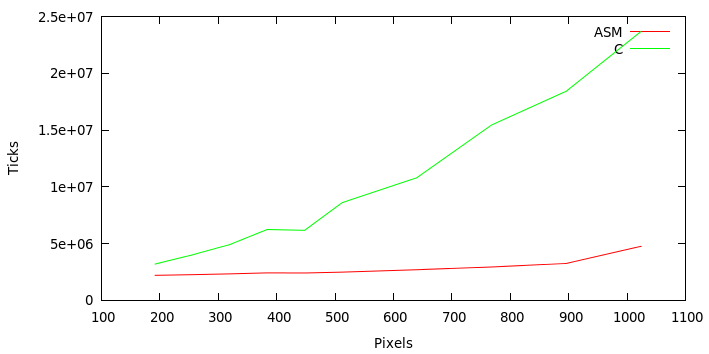
\includegraphics[scale=0.66]{imagenes/smalltilesC.png}
	\caption{Comparación de los tiempos de ejecución de cada implementación}
	\label{smalltiles_asmvsc}
  \end{center}
\end{figure}

Como se puede apreciar en la figura~\ref{smalltiles_asmvsc}, hay una clara diferencia entre el tiempo de ejecución del filtro en lenguaje ensamblador frente a su análogo en C (sin optimizar). Particularmente, la medición de la implementación en lenguaje ensamblador es un 95\% menor. Sin embargo, al aplicar las optimizaciones del compilador, la diferencia se reduce abruptamente, siendo la implementación compilada con el flag \textit{O1} un 65\% menor que la implementación sin optimizaciones; y al aplicar todas las optimizaciones posibles, se obtiene una diferencia del 90\%, acercándolo a los tiempos de ejecución de la implementación en lenguaje ensamblador. Creemos que las optimizaciones hacen mucha diferencia porque la implementación en C hace uso de varios punteros en cada iteración (siempre haciendo el mismo cálculo con respecto al índice), por lo que le da lugar al compilador a varias mejoras.

\subsubsection{Experimentacion}
\textbf{Hipótesis}
\newline
La implementación en lenguaje ensamblador consiste únicamente de ejecutar la instrucción \textit{shuffle} sobre los pixeles a procesar, utilizando un inmediato de 8 bits para reordenar los datos. Dado que el reordenamiento de los datos no es complicado, se lo puede reemplazar fácilmente utilizando \textit{shift} y las operaciones \textit{insert} y \textit{extract}, de manera tal de no perder información al realizar el \textit{shift}.

Si bien es de esperar que la operación \textit{shift} consuma menos tiempo de ejecución que \textit{shuffle}, ya que simplemente es un corrimiento de bits, queremos analizar si en conjunto con las operaciones \textit{insert} y \textit{extract} es posible obtener un mejor rendimiento. Dado que tanto \textit{shuffle} como \textit{insert} y \textit{extract} utilizan bits de control para el reordenamiento de datos, suponemos que utilizan una lógica o unidades de hardware similares, y los tiempos de ejecución no deberían variar mucho.

\textbf{Resultados}

Para lograr analizar la diferencia entre las instrucciones, medimos los tiempos de ejecución de ambas implementaciones en lenguaje ensamblador (según lo descrito al principio del trabajo práctico) y las comparamos frente a la medición de control (implementación en C con el flag \textit{O3}). Sin embargo, al ejecutarlo sobre datos de entrada más chicos, obtuvimos resultados diferentes.
\\
\begin{figure}[H]
  \begin{center}
	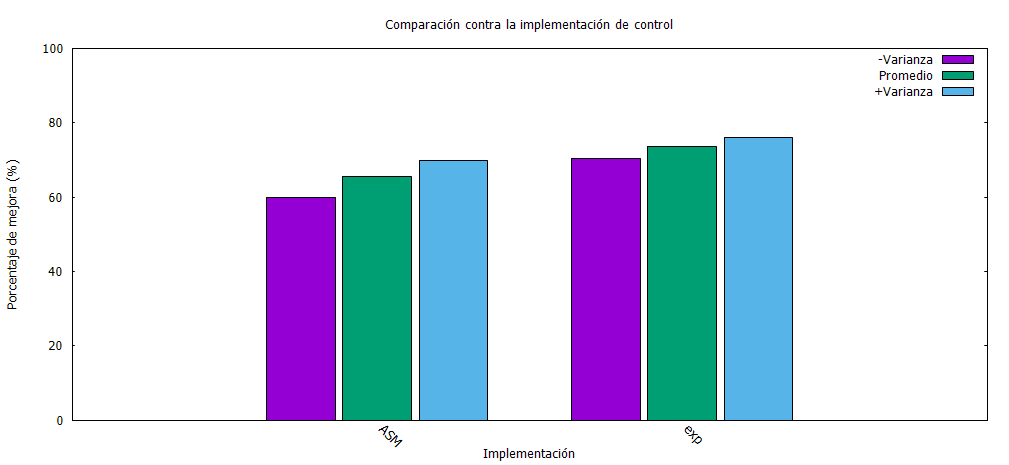
\includegraphics[scale=0.66]{imagenes/smalltilesExpC}
	\caption{Comparación de los tiempos de ejecución del experimento}
	\label{smalltiles_chico}
  \end{center}
\end{figure}

En este caso, se midieron los tiempos de ejecución sobre una imagen de tamaño 256x256 pixels. Como se puede observar, el uso de las instrucciones \textit{insert} y \textit{extract} resultó ser más eficiente, hasta un 8\% mejor que la implementación regular en lenguaje ensamblador (utilizando \textit{shuffle}). Luego, al realizar las mediciones sobre el tamaño de imagen elegido (768x768 pixels) se obtuvieron los siguientes resultados:
\\
\begin{figure}[H]
  \begin{center}
	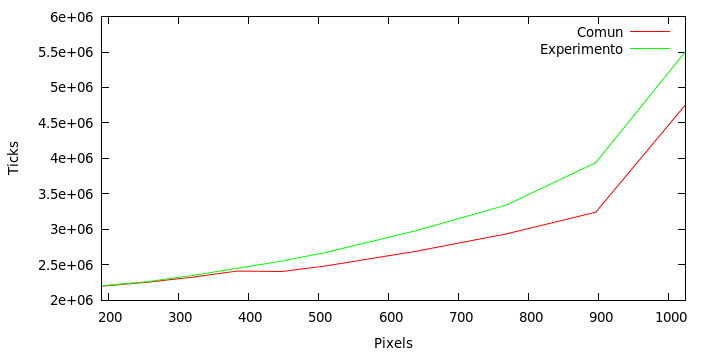
\includegraphics[scale=0.66]{imagenes/smalltilesExp.png}
	\caption{Comparación de los tiempos de ejecución del experimento}
	\label{smalltiles_exp}
  \end{center}
\end{figure}

Tal como se muestra en la figura~\ref{smalltiles_exp}, los resultados se invirtieron: la instrucción \textit{shuffle} resultó ser más eficiente que su análogo con \textit{insert} y \textit{extract}, hasta un 20\% mejor. Desconocemos por qué para datos de entrada más pequeños el rendimiento es incluso mejor bajo el uso de \textit{insert} y \textit{extract}; probablemente el uso de una mayor cantidad de instrucciones (por más leve que sea la diferencia) tiene su peso cuando se procesan más datos. Sin embargo, podemos concluir que, en líneas generales, es preferible utilizar \textit{shuffle} para reordenar datos.

\newpage
\subsection{Rotar}
\subsubsection{Implementación}
Este filtro lo que hace es simplemente rotar los valores de los colores en los pixeles. Lo implementamos en muy pocas líneas en lenguaje ensamblador gracias a que utilizamos la instrucción \textit{shuffle} junto a una máscara (escrita como constante en memoria) que indica la nueva posición de cada valor en el píxel de la imagen destino. Por lo tanto, lo único que se realiza en cada iteración es la carga de la imagen de memoria en un registro, ejecutar la instrucción \textit{shuffle} y almacenar el registro en la posición de memoria del puntero a la imagen destino. 
\\Como los valores en los pixeles no son alterados de ninguna forma, no hay pérdida de precisión alguna.\\

Se itera sobre la imagen columna por columna, y, una vez que se terminó de recorrer una fila, se decrementa el contador que contiene la cantidad de filas a recorrer. De esta manera, una vez que dicho contador llegó a cero, se terminó de recorrer la imagen. Como se opera de a 4 pixeles por vez, se divide la cantidad de columnas (que están en pixeles) por cuatro y los punteros avanzan de a 16 bytes. No se puede operar de a más pixeles por vez porque cada uno ocupa 32 bits, entonces solo se pueden almacenar cuatro de ellos por vez en los registros de SIMD.\\


La implementación realizada en C itera sobre la imagen con dos ciclos anidados (avanzando por columnas), de a un píxel por vez. Simplemente rota los valores de los pixeles en la imagen destino. Si bien las operaciones se realizan de manera muy similar a la implementación en lenguaje ensamblador, esta última recorre la imagen más rápido al procesar de a 4 pixeles por iteración, por lo que el rendimiento debería ser mayor.\\

\begin{figure}[H]
  \begin{center}
	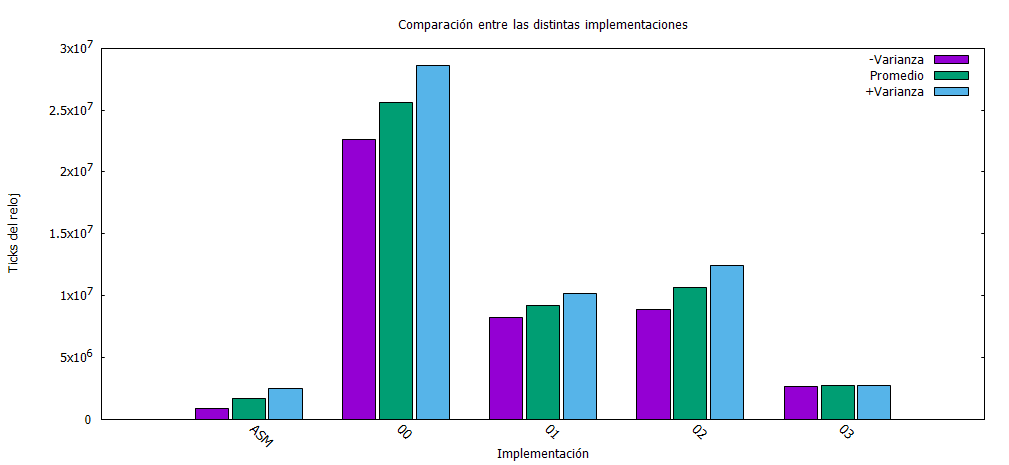
\includegraphics[scale=0.66]{imagenes/rotarC.png}
	\caption{Comparación de los tiempos de ejecución de cada implementación}
	\label{rotar_asmvsc}
  \end{center}
\end{figure}

Como se puede observar en la figura~\ref{rotar_asmvsc}, la cantidad de \textit{ticks} de reloj necesarios para ejecutar el mismo filtro en su implementación en C sin optimizar es considerablemente mayor a aquellos necesarios para ejecutar el filtro en su implementación en lenguaje ensamblador, siendo la medición de esta última un 90\% menor. Por otro lado, la implementación en C optimizada mediante el flag \textit{O1} resultó ser un 63\% mejor que aquella sin optimizar y, casualmente, frente a la optimización mediante \textit{O2} resultó ser un 13\% mejor. Sin embargo, al aplicarle todas las optimizaciones posibles del compilador, los tiempos de ejecución se empiezan a asemejar a aquellos de la implementación en lenguaje ensamblador, resultando ser un 70\% mejor que su análoga con el flag \textit{O1}.

\subsubsection{Experimentación}
\textbf{Hipótesis}
\newline
La instrucción principal de este filtro, como mencionamos anteriormente, es \textit{shuffle}. En esta experimentación queremos probar lo que ocurre si hacemos la rotación de valores (es decir, lo que se realiza con la instrucción \textit{shuffle}) de manera manual, simplemente desempaquetando y empaquetando los valores en las nuevas posiciones. Esto implica escribir más instrucciones y realizar un código más ilegible.
\\Como la cantidad de instrucciones ha aumentado considerablemente, creemos que el tiempo de ejecución será mayor, a pesar de que sean (probablemente) menos costosas que la operación \textit{shuffle}. Aun así, debería ser menor a la implementación en C. 
\newline

\textbf{Resultados}
\\Se realizó una medición de la cantidad de \textit{ticks} de reloj del CPU que conllevó ejecutar el filtro según lo descrito al principio del informe y se lo comparó frente a su versión de control (la implementación en C compilada con el flag \textit{O3}).

\begin{figure}[H]
  \begin{center}
	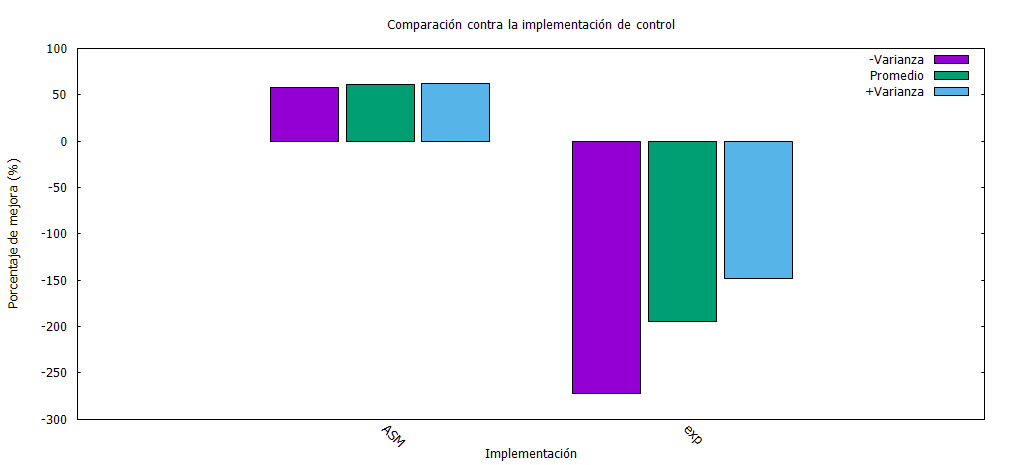
\includegraphics[scale=0.66]{imagenes/rotarExp.png}
	\caption{Comparación de los tiempos de ejecución}
	\label{rotar_exp}
  \end{center}
\end{figure}

Los resultados coinciden con lo esperado, donde los tiempos de ejecución del filtro operando con la instrucción \textit{shuffle} son menores al resto (hasta un 50\% mejor que la implementación de control), pero los tiempos de ejecución empaquetando y desempaquetando son mucho mayores, hasta un 200\% peor en promedio. Concluimos que el empaquetado y desempaquetado de datos conlleva un costo mayor para reordenar datos a su equivalente utilizando la instrucción \textit{shuffle}.

\newpage

\subsection{Pixelar}
\subsubsection{Implementación}
Como el filtro necesita la información de dos filas para realizar el promedio, recorremos tanto la imagen fuente como la imagen destino con dos punteros. Estos se mueven de forma paralela, es decir, en las mismas columnas pero en filas consecutivas. Al trabajar de esta forma y utilizando instrucciones SIMD podemos aplicar los cambios a ocho pixeles a la vez (cuatro por punteros).

Para no perder precisión, todas las operaciones necesarias para obtener los promedios se realizan en enteros. Una vez calculados (uno por grupo de 4 pixeles), se reemplazan los valores originales de los pixeles en la imagen destino por el valor promedio correspondiente.
\\

Se itera sobre la imagen columna por columna, y, una vez que se terminaron de recorrer las dos filas paralelas, se decrementa el contador que contiene la mitad de la cantidad total de filas a recorrer. De esta manera, una vez que dicho contador llegó a cero, se terminó de recorrer la imagen. Como se opera de a 4 pixeles por puntero, se divide la cantidad de columnas (que están en pixeles) por cuatro y los punteros avanzan de a 16 bytes. A su vez, cuando se terminan de recorrer las filas, los punteros avanzan la cantidad de columnas multiplicado por cuatro (bytes), saltándose cada puntero una fila. No se puede operar de a más pixeles por vez porque cada uno ocupa 32 bits, por lo que solo se pueden almacenar cuatro de ellos a la vez en los registros de SIMD.
\\

La implementación realizada en C itera sobre la imagen con dos ciclos anidados (avanzando por columnas) de a 4 pixeles por vez, avanzando de a dos columnas y dos filas a la vez. Simplemente se calcula el promedio en cuatro pixeles y se coloca este valor en la imagen destino en las posiciones de los pixeles procesados. Si bien las cuentas se realizan de manera muy similar a la implementación en lenguaje ensamblador, esta última recorre la imagen más rápido al procesar de a 8 pixeles por iteración, por lo que el rendimiento debería ser mayor. Las mediciones se realizaron según lo descrito al principio del informe.
\\
\begin{figure}[H]
  \begin{center}
	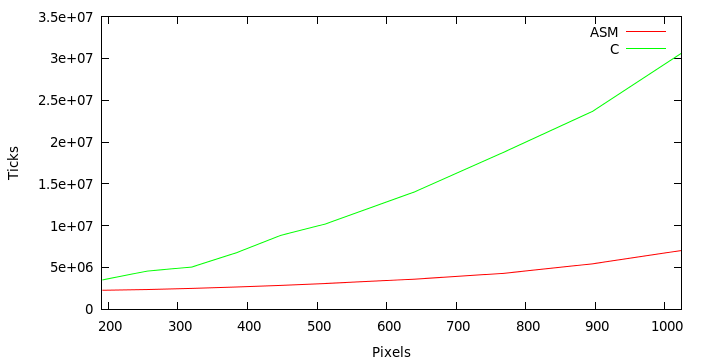
\includegraphics[scale=0.66]{imagenes/pixelarC.png}
	\caption{Comparación de los tiempos de ejecución de cada implementación}
	\label{pixelar_asmvsc}
  \end{center}
\end{figure}

Como se puede observar en la figura~\ref{pixelar_asmvsc}, la cantidad de \textit{ticks} de reloj necesarios para ejecutar el mismo filtro en su implementación en C sin optimizar es considerablemente mayor a aquellos necesarios para ejecutar el filtro en su implementación en lenguaje ensamblador (el cual es un 88\% menor), como se suponía. Al aplicar las optimizaciones del compilador, los tiempos de ejecución mejoran; al compilar con el flag \textit{O1}, se obtuvieron resultados del 50\% mejores con respecto a la implementaicón sin optimización, con el flag \textit{O2} la mejora asciende al 70\%. Curiosamente, el flag \textit{O3} no solo no mejora el tiempo de ejecución, sino que lo empeora en un 13\% con respecto al flag \textit{O2}, por lo que se deduce que las optimizaciones extras incluídas en el mismo fueron futiles.

\subsubsection{Experimentación}
\textbf{Hipótesis}


Dentro de las series de operaciones que ejecuta el filtro, existe una división entera que efectuamos con la instrucción \textit{psrld}. En esta experimentación queremos ver la diferencia, tanto en tiempo como en precisión, al utilizar una división de punto flotante. Entendemos que en este caso no tiene sentido utilizarla, porque los decimales que perdemos al utilizar la división entera los ibamos a descartar de todas formas, ya que la información en los pixeles se encuentra en enteros. Aún así, nos interesa ver las diferencias entre ambos métodos. Suponemos que la diferencia en rendimiento no debería variar mucho, ya que la división en punto flotante se realiza a través de una tabla \textit{hardcodeada}, y analizaremos la variación en la precisión (la cual debería ser peor para la división en punto flotante).
\newline

\textbf{Resultados}

Se realizó una medición de la cantidad de \textit{ticks} de reloj del CPU que conllevó ejecutar el filtro, según lo descrito al principio del informe.
\\
\begin{figure}[H]
  \begin{center}
	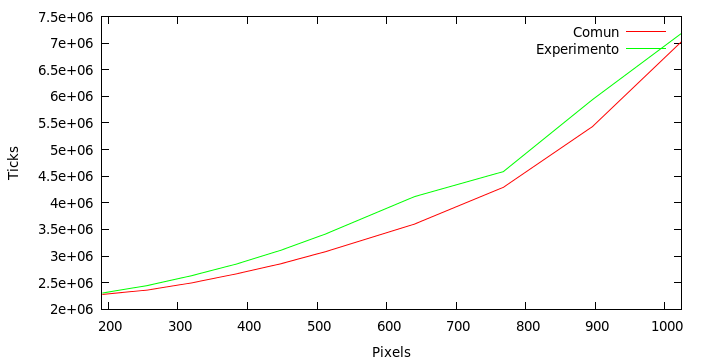
\includegraphics[scale=0.66]{imagenes/pixelarExp.png}
	\caption{Comparación de los tiempos de ejecución}
	\label{pixelar_exp}
  \end{center}
\end{figure}

Los resultados indican que, si bien existe una tabla \textit{hardcodeada} para las operaciones costosas como multiplicación y división en punto flotante, su costo sigue siendo mayor a aquél de operar la división \textit{shifteando}, pero se mantiene una mejora notable frente a la implementación de control. El costo insumido por realizar operaciones de punto flotante es de un 4\% mayor con respecto al uso del \textit{shift}.

Una vez determinado que insume un mayor costo la operación con punto flotante, falta analizar la diferencia en la precisión.

Para analizar qué tanta diferencia hay entre un resultado y otro, utilizamos la herramienta \textit{bmpdiff}, generando imágenes que muestran la diferencia píxel a píxel para cada componente. El parámetro epsilon de la herramienta \textit{bmpdiff} se fijó en cero.
\\
\begin{figure}[H]
  \begin{center}
	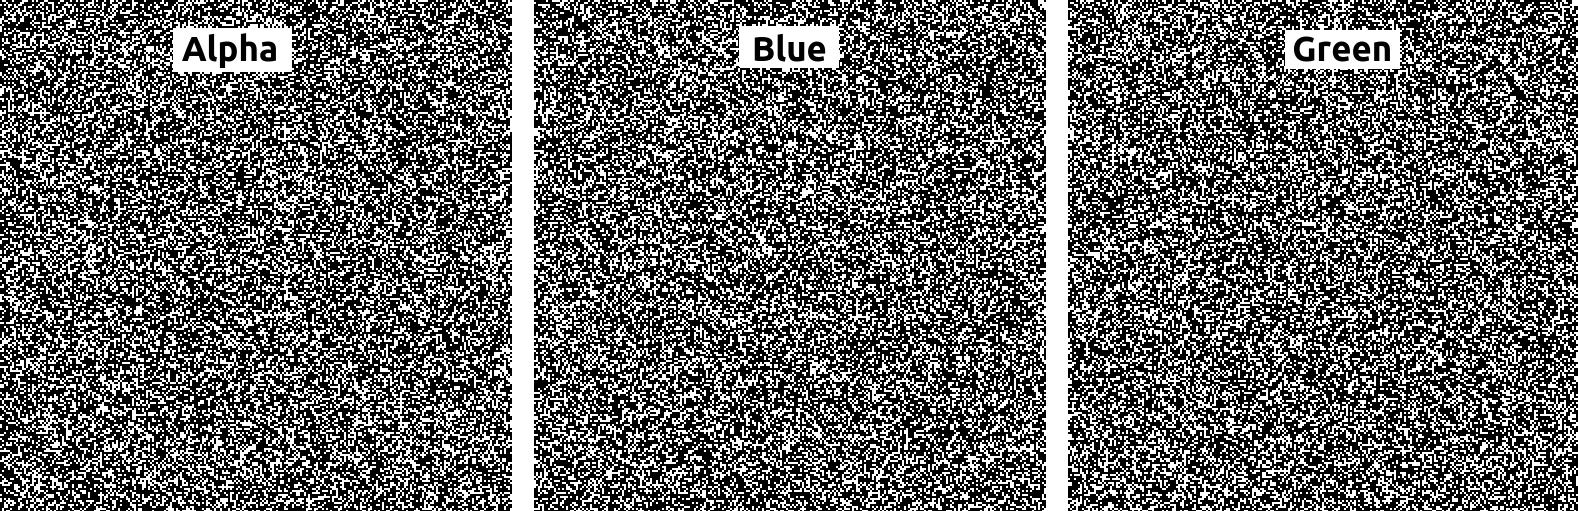
\includegraphics[scale=0.40]{imagenes/pixelardiffExp.jpeg}
	\caption{Diferencia píxel a píxel para cada componente}
	\label{pixelar_diff}
  \end{center}
\end{figure}

Como se puede observar, las diferencias en la imagen son uniformes, lo que confirma que el color no tuvo incidencia en las operaciones. Si bien parecen ser muchos los pixeles con distintos valores, la diferencia es prácticamente nula: al ejecutar \textit{bmpdiff} una vez más pero con el parámetro epsilon en 1 (es decir, permitiendo que haya un margen de error de $+/-$ uno para cada color) se obtuvieron imágenes en negro para todas las componentes. En otras palabras, solo difieren en uno cada componente de cada píxel. Luego, podemos concluir que no se produce una pérdida de precisión por utilizar uno u otro método, sino una diferencia en términos de redondeo.

\newpage
\subsection{Combinar}
\subsubsection{Implementación}
Ya que el filtro se ejecuta sobre el reflejo vertical de la imagen fuente, en lenguaje ensamblador se mantiene como invariante un puntero a la imagen invertida. Es decir, a medida que se recorre la matriz de la imagen fuente, este puntero la recorre de atrás hacia delante. Por lo tanto, avanza restándole posiciones de memoria. Por otro lado, como recorre de atrás hacia delante, levanta los pixeles de memoria de manera invertida, por lo que en cada iteración del ciclo, luego de levantar los pixeles, se reordenan de manera que coincidan vectorialmente con aquellos contenidos en el registro que opera sobre la matriz comúnmente (es decir, de delante hacia atrás).
\\

Para no perder precisión, antes de realizar la resta entre pixeles, se extiende cada componente del píxel a un entero de 32 bits y se hacen todas las operaciones intermedias operando como \textit{floats}. Además, como la cuenta incluye el uso de constantes, las mismas se guardan en memoria como datos de solo lectura. Para no perder rendimiento levantándolas en cada iteración del ciclo, se guardan en un registro específico antes de empezar a recorrer la imagen.

Se itera sobre la imagen columna por columna, y, una vez que se terminó de recorrer una fila, se decrementa el contador que contiene la cantidad de filas a recorrer. De esta manera, una vez que dicho contador llegó a cero, se terminó de recorrer la imagen. Como se opera de a 4 pixeles por vez, se divide la cantidad de columnas (que están en pixeles) por cuatro y los punteros avanzan de a 16 bytes. No se puede operar de a más pixeles por vez porque cada uno ocupa 32 bits, entonces solo se pueden almacenar cuatro de ellos por vez en los registros de SIMD.
\bigskip

La implementación realizada en C itera sobre la imagen con dos ciclos anidados (avanzando por columnas), de a un píxel por vez. Las operaciones se realizan con una variable auxiliar de tipo \textit{float} y luego se castea la misma al tipo de dato de la estructura correspondiente al color del píxel (\textit{unsigned char}). Si bien las cuentas se realizan de manera muy similar a la implementación en lenguaje ensamblador, esta última recorre la imagen más rápido al procesar de a 4 pixeles por iteración, por lo que el rendimiento debería ser mayor. 
\\
\begin{figure}[H]
  \begin{center}
	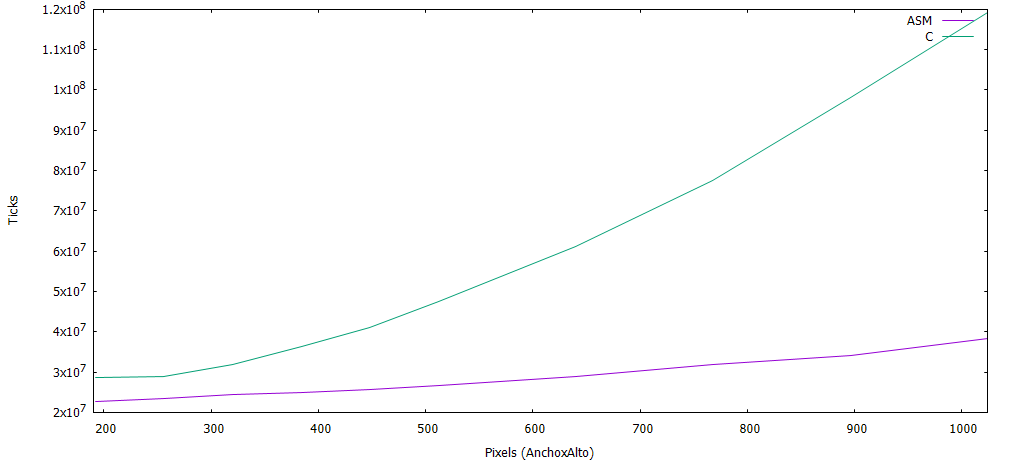
\includegraphics[scale=0.6]{imagenes/combinarC.png}
	\caption{Comparación de los tiempos de ejecución de cada implementación}
	\label{combinar_asmvsc}
  \end{center}
\end{figure}

Como se puede observar en la figura~\ref{combinar_asmvsc}, la cantidad de \textit{ticks} de reloj necesarios para ejecutar el filtro en su implementación en C es mayor a su análoga en lenguaje ensamblador, incluso utilizando las optimizaciones del compilador. La diferencia es más notoria que en otros filtros, ya que, porcentualmente, la medición de la implementación en lenguaje ensamblador es un 83\% menor que la medición de la implementación con la mayor cantidad de optimizaciones del compilador (\textit{O3}). La implementación con el flag \textit{O2} resultó ser un poco menor a aquella con el flag \textit{O3}, por lo que se deduce que las optimizaciones extra que conlleva \textit{O3} frente a \textit{O2} no propician ninguna mejora (y resulta en un rendimiento ligeramente menor) en este filtro. Por otra parte, la diferencia entre estos últimos y \textit{O1} es casi del 20\%, mientras que frente a la implementación sin optimización resultaron ser un 52\% mejor. Desconocemos por qué para este filtro en particular las optimizaciones del compilador no mejoraron el rendimiento en la misma proporción que para los demás, pero podemos suponer que se debe a la cantidad de \textit{casteos} necesarios que se realizan en el código en C.

Las mediciones se realizaron según lo descrito al principio del informe, con un parámetro \textit{alpha} de 128.
\subsubsection{Experimentación}
\textbf{Hipótesis}

Ya que el filtro consta de ejecutar una serie de operaciones, la mayor complejidad del mismo se encuentra en las cuentas que hay que realizar. Si bien la suma y resta de enteros no insume prácticamente ningún costo, dentro de las operaciones a realizar se encuentra una multiplicación con valores de punto flotante (\textit{alpha}) y la división por 255.0. Ya que \textit{alpha} representa un valor comprendido en [0.00;255.0], si se lo interpreta como un entero, el truncamiento no representa una pérdida de precisión muy importante, y el rendimiento obtenido debería compensar tal pérdida. Así mismo, se puede realizar algo similar con la división por 255.0. Si bien la división por enteros es costosa, es posible dividir el resultado parcial obtenido por 256 en lugar de 255. La operación no insume un mayor costo porque simplemente consta de \textit{shiftear} los bits, en lugar de realizar una división propiamente dicha. Además, ya que la operación se realizaría únicamente con enteros, no es necesario hacer \textit{casteos} intermedios entre punto flotante y enteros, los cuales son muy costosos.
\newline
\\
\textbf{Resultados}

Se realizó una medición de la cantidad de \textit{ticks} de reloj del CPU que conllevó ejecutar el filtro según lo descrito al principio del informe, comparándolo con la implementación en C de control (aquella compilada con el flag \textit{O2}, según lo visto anteriormente).
\\
\begin{figure}[H]
  \begin{center}
	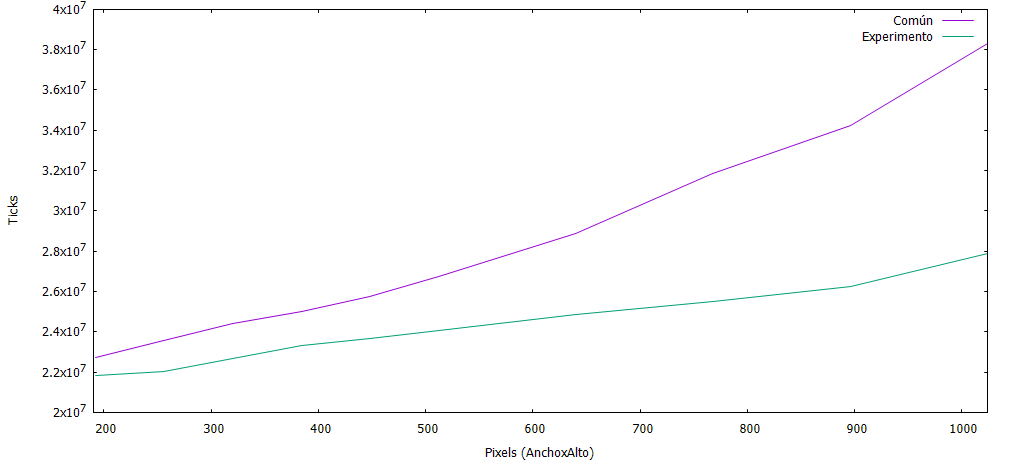
\includegraphics[scale=0.6]{imagenes/combinarExp.png}
	\caption{Comparación de los tiempos de ejecución}
	\label{combinar_exp}
  \end{center}
\end{figure}

Los resultados condicen con lo esperado, donde los tiempos de ejecución del filtro operando únicamente con enteros son menores a aquellos utilizados para operar con punto flotante.

Como se puede observar en la figura~\ref{combinar_exp}, la mejora frente a la implementación de control es del 85\%, un 4\% mejor que la implementación común en lenguaje ensamblador. Queda claro que el rendimiento mejora al operar con enteros, dado a la complejidad de las operaciones en punto flotante, pero falta analizar en cuánto difiere la precisión.
\bigskip

Para analizar qué tanta diferencia hay entre un resultado y otro, utilizamos la herramienta \textit{bmpdiff}, generando imágenes que muestran la diferencia píxel a píxel para cada componente. Las imágenes se obtuvieron corriendo el filtro con el parámetro \textit{alpha} de valor 127.484, para realzar las diferencias por pérdida de precisión. El parámetro epsilon de la herramienta \textit{bmpdiff} se fijó en cero.
\\
\begin{figure}[H]
  \begin{center}
	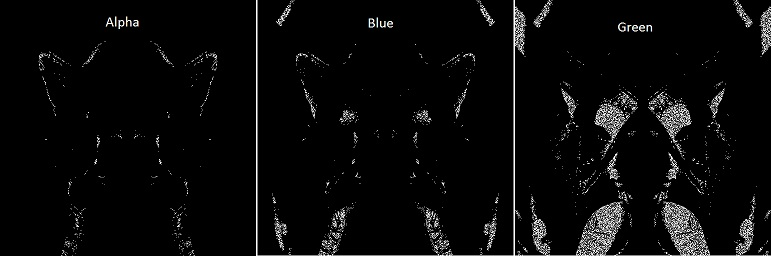
\includegraphics[scale=0.6]{imagenes/diffExp.jpg}
	\caption{Diferencia píxel a píxel para cada componente}
	\label{combinar_diff}
  \end{center}
\end{figure}

Como se puede observar, la mayor diferencia se obtiene en la componente verde, mientras que no hubieron diferencias en la componente alpha. Si bien parecen ser varios los pixeles con distintos valores, la diferencia es prácticamente nula: al ejecutar \textit{bmpdiff} una vez más pero con el parámetro epsilon en 1 (es decir, permitiendo que haya un margen de error de $+/-$ uno para cada color) se obtuvo imágenes en negro para todas las componentes. En otras palabras, la diferencia en la precisión es mínima, ya que solo difieren en uno cada componente de cada píxel, mientras que la mejora en rendimiento es notable, especialmente para imágenes de mayor tamaño. Por lo tanto, se concluye que es preferible utilizar la implementación con enteros ya que la única diferencia se encuentra en el redondeo de los valores.

\newpage

\subsection{Colorizar}
\subsubsection{Implementación}

El filtro Colorizar trabaja con los valores máximos de los colores de aquellos pixeles que se encuentren alrededor del píxel a procesar, incluyéndolo. Por esta razón, se mantuvo un puntero a la fila anterior y posterior del píxel a procesar, de manera tal de poder aprovechar las instrucciones de SIMD para realizar varias comparaciones simultáneamente. Por otro lado, como las operaciones a realizar incluyen el uso de constantes, las mismas se cargaron en memoria (en la sección de datos de solo lectura) y luego a los registros al inicio del programa. Además, por enunciado, la primera y última fila, así como la primera y última columna, no se procesan. Por lo tanto, el puntero a la imagen destino comienza una fila y una columna más adelante. Lo mismo ocurre para el puntero de la imagen fuente que contiene los pixeles a procesar. 

Debido a que no se procesa la primera y última columna (siendo la cantidad total de columnas múltiplo de cuatro), y solo se pueden realizar comparaciones de a cuatro pixeles por vez, el algoritmo implementado en lenguaje ensamblador procesa de a dos pixeles por iteración.

Luego de obtener los valores máximos de cada color de los pixeles a procesar y sus vecinos, se comparan entre ellos generando máscaras. Estas mismas máscaras aprovechan el valor \textit{true} de las comparaciones interpretándolas como un $-1$ y, luego de obtener su complemento, agregando el valor $1$ donde haya ceros. De esta manera, al multiplicar por el registro que contiene al parámetro $\alpha$, se obtiene $-\alpha$ en aquellos lugares donde la comparación haya resultado falsa y $\alpha$ en aquellos lugares donde la comparación haya resultado verdadera. Luego solo resta sumar por la constante $1.0$ cargada previamente en un registro. 

Para obtener los mínimos entre los resultados obtenidos y el valor $255$, se realiza una operatoria muy similar utilizando máscaras junto con la operación lógica AND y luego sumando. El valor $alpha$ original de los pixeles es copiado al resultado una vez realizadas las operaciones.
\bigskip

En el caso de la implementación realizada en C, la iteración sobre la matriz opera de manera muy similar, salteando la primera y última fila y la primera y última columna de cada fila, con la diferencia de que se procesa de a un píxel por vez. Además, para buscar el máximo, se realiza otro bucle iterando sobre los vecinos del píxel, por lo que se espera que la diferencia de rendimiento entre una implementación y otra sea considerable (ya que realiza bastantes más accesos a memoria que la implementación en lenguaje ensamblador).

Solo se varió el tamaño de las imágenes a probar porque, si bien los máximos dependen del valor de los colores, las comparaciones se efectúan independientemente de sus valores, y la operación a realizar (suma o resta) según los resultados de las mismas es equivalente en términos de rendimiento.
\\
\begin{figure}[H]
  \begin{center}
	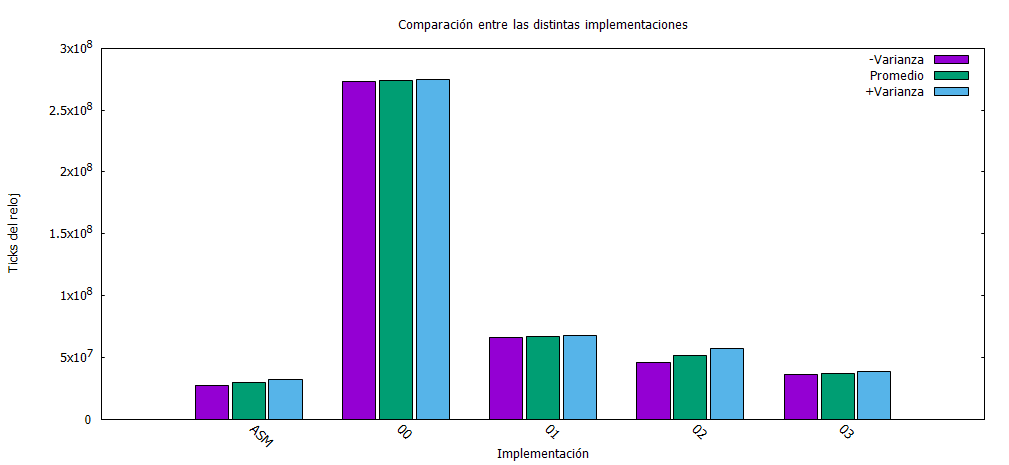
\includegraphics[scale=0.6]{imagenes/colorizarC.png}
	\caption{Comparación entre las distintas implementaciones}
	\label{colorizar_asmvsc}
  \end{center}
\end{figure}

Como se puede observar en la figura~\ref{colorizar_asmvsc}, la diferencia entre la implementación en lenguaje ensamblador y aquella compilada en C sin optimizaciones es muy grande, siendo la medición promedio de la primera un 90\% menor. Sin embargo, una vez aplicadas algunas optimizaciones, la diferencia se achica abruptamente (la diferencia con la implementación compilada con el flag \textit{O1} es casi del 80\%). Por otro lado, la implementación con el flag \textit{O3} es aproximadamente un 45\% mejor que aquella con el flag \textit{O1}.

Suponemos que la diferencia entre la implementación sin optimizar y la optimizada es más notable que en otros filtros por la cantidad de condiciones y líneas de código que se encuentran presentes en la implementación en C, por lo que da lugar a una mayor posibilidad de optimización.
\\
\subsubsection{Experimentación}
\textbf{Hipótesis}

Dado que el filtro se caracteriza por buscar los máximos en un cuadrado alrededor del píxel a procesar, muchos resultados se solapan. Es decir, los máximos de cada columna se calculan más de una vez. Si bien esto no representa un problema para la implementación en lenguaje ensamblador (ya que las comparaciones se realizan de manera vectorial y los accesos a memoria no se reducen), para la implementación en C se puede reducir considerablemente los accesos a memoria si se reusan los resultados, manteniendo los resultados parciales (como una suerte de programación dinámica). De esta manera, excepto para la primera iteración de cada fila, ya se consiguieron los máximos de dos de las tres columnas a evaluar.

Almacenando estos resultados parciales, se reducen los accesos a memoria en un orden no menor, dado que solo es necesario calcular el máximo de la columna siguiente al píxel a procesar. En total, la cantidad de accesos a memoria deberían reducirse en $2/3$ (aproximadamente, ya que para la primera iteración de cada fila sigue siendo necesario calcular los máximos de las tres columnas).

Los accesos a memoria deberían conformar una parte considerable del costo insumido por la implementación en C, por lo que se espera que, al reducirlos, la diferencia de tiempos entre la implementación en ensamblador y la implementación en C sea menor a aquella de los demás filtros (dado que en este filtro se procesa de a dos en lugar de a cuatro).
\\

\textbf{Resultados}

Para analizar lo dicho, se ejecutó ambas implementaciones en C de la manera descrita al principio del trabajo práctico y se comparó ambos resultados, utilizando el flag \textit{O3} para la compilación.
\\
\begin{figure}[H]
  \begin{center}
	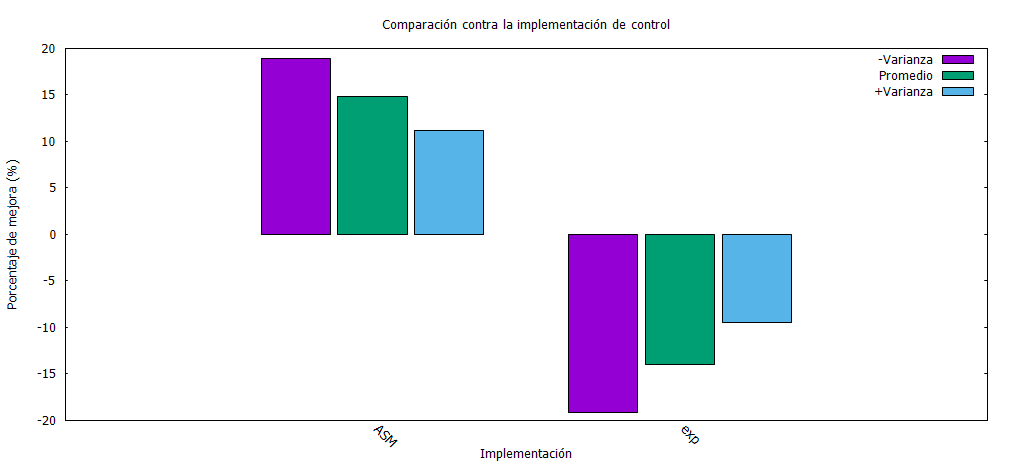
\includegraphics[scale=0.6]{imagenes/colorizarExp.png}
	\caption{Comparación entre las distintas implementaciones en C}
	\label{colorizar_exp}
  \end{center}
\end{figure}

Como se puede observar en la figura~\ref{colorizar_exp}, los tiempos de ejecución de la implementación del experimento resultaron ser peores que aquellos de la implementación de control, resultando ser aproximadamente un 15\% más lento. Sin embargo, frente a la implementación sin optimizaciones, el experimento dio resultados positivos. Por lo tanto, podemos concluir que dentro de las optimizaciones del compilador ya se incluye una mecánica similar a la propuesta en el experimento, almacenando los resultados parciales. Suponemos que la implementación del experimento resultó ser incluso peor porque posee más líneas de código.

\end{document}
